\documentclass[]{article}
\usepackage{geometry}
 \geometry{
 a4paper,
 total={170mm,257mm},
 left=20mm,
 top=20mm,
 }
\usepackage{graphicx}
\usepackage{subcaption}

\usepackage[justification=centering]{caption}
\usepackage[hidelinks]{hyperref}
\usepackage{enumitem}
\usepackage[utf8]{inputenc}
\usepackage{float}
\DeclareTextFontCommand{\helvetica}{\fontfamily{phv}\selectfont}
\setlength{\parindent}{4em}
\setlength{\parskip}{1em}
\linespread{1.5}

\usepackage[table]{xcolor}



\title{PAC1 Plà de treball}
\date{18 de Març 2019}
\author{Vasyl Druchkiv \\ Estudiant de Màster de Bioestadística i Bioinformàtica}
\renewcommand{\contentsname}{Índice}
\usepackage{setspace}

\begin{document}
\maketitle
\makeatletter
\renewcommand{\@seccntformat}[1]{}
\makeatother
\begin{spacing}{0.1}
\tableofcontents
\end{spacing}

\section{Context i justificació del treball}
\subsection{Descripción general}
El treball consistirà en el desenvolupament d'una aplicació per dur a terme l'anàlisi de les rutes (\textit{Pathway analysis}). Amb les rutes entenem un conjunt de gens que actuen junts per dur a terme un procès biològic. Així doncs aquest anàlisi permet donar més sentit a una expressió genètica diferencial entre les proves biològiques d'interès. Recordem que recents avenços tecnològics permeten mesurar els nivells d'expressió en una gran quantitat de gens, cosa que implica una gran quantitat de dades. Al nivell dels gens individuals es poden fer servir mètodes estadístics per comprovar si les diferències en les expressions entre els grups (proves biològiques) són estadísticament significatives. Per dotar encara de més sentit aquesta anàlisi és necessari agregar els resultats al nivell més raonable com ara al nivell de les rutes. Al final el que volem és comprovar si hi ha diferències estadísticament significatives entre les proves no al nivell dels gens perticulars sinó al nivell de les rutes. Tan com en el cas dels gens particulars també en el nivell de les rutes s'han desenvolupat mètodes estadístics específics \cite{khatri2012ten}. En aquest treball vull analitzar quins mètodes són i quins tenen més avantatges que d'altres. A part d'aquest component més biològic i teòric del treball buscaré la possibilitat d'implementar aquests mètodes d'anàlisi en una aplicació intuïtiva i d'un ús fàcil a la qual qualsevol científic que no disposi dels coneixements informàtics suficients per fer aquesta anàlisi podrà accedir gratuïtament. La plataforma que utilitzaré per crear l'aplicació és l'eina Shiny de Rstudio \cite{Shiny}.  La feina doncs consistirà en la cerca dels paquets de Bioconductor que inclouen els mètodes per l'anàlisi de les rutes, selecció dels paquets més apropiats i la seva integració en una aplicació Shiny amb una interfície atractiva. Ja he fet una cerca previa sobre els paquets-canditats per una applicació. Aquests paquets són: ReactomePA, GAGE, clusterProfiler. Uns dels objectius és però fer una cerca dels paquets més exhaustiva.

\subsection{Justificació del TFM}
La justificació d'aquest tema ve de dues fonts diferents: d'una banda tinc un interès personal i d'altra banda entenc la importància de la meva aportació per a la comunitat científica. El meu interès personal és degut al fet que durant el màster he fet servir àmpliament el programa R però no he arribat a conèixer bé la creació d'una aplicació estadística amb Shiny. Per completar aquesta deficiència i entenent que aquesta eina és útil per al méu desenvolupament professional he buscat el tema que en requeria l'ús. Tot i la importància de l'anàlisi de les rutes, al meu saber encara no existeix cap aplicació Shiny que integri paquets diversos i molt efectius de Bioconductor. L'ús d'aquests paquets requereix coneixements informàtics i estadístics específics i per tant és difícilment accecible per la gran part de la comunitat scientífica. Encara que hi ha ja plataformes gratuïtes que ofereixen l'anàlisi de les rutes \cite{reimand2019pathway} crec que val la pena desenvolupar una eina més que seria de codi obert.

\section{Objectius}
\subsection{Objectius generals}
\begin{enumerate}
\item Identificar els objectius i mètodes de l'anàlisi de les rutes (Bio/Stat)
\item Identificar els paquets de Bioconductor en R que s'aproximin als mètodes (Info)
\item Desenvolupar l'aplicació Shiny  amb els paquets escollits per aproximar el resultat als objectius de l'anàlisi de les rutes  (Info)
\end{enumerate}

\subsection{Objectius específics}
\begin{enumerate}
\item Biologia/Estadística
\begin{enumerate}
\item Buscar literatura sobre l'anàlisi de rutes
\begin{itemize}
\item Quins mètodes hi ha? Enumerar-los i explicar-los, especialment els tests estadístics.
\begin{itemize}
\item Els tests sobre uns llistats de gens diferencialment expressats $\rightarrow$ Test de distribució hipergeomètrica?
\item Els tests sobre tots els gens d'experiment $\rightarrow$ GSEA $\rightarrow$  Enrichment Score $\rightarrow$ Permutació de gens/mostres? $\rightarrow$ Kolmogorov Test?
\end{itemize}
\item Quines bases de dades es fan servir?
\item Què signifiquen els diagrames més usats en l'anàlisi de rutes?
\begin{itemize}
\item Barplots
\item Enrichment Maps
\item Barplots/Dot plots
\item GSEA plots
\item Altres?
\end{itemize}
\end{itemize}
\item Identificar les aplicacions existens i investigar què ofereixen
\item Analitzar els vignettes dels paquets de Bioconductor i provar-ne el seu ús localment amb R
\begin{itemize}
\item RectomePA
\item GAGE
\item clusterProfiler
\item Altres?
\end{itemize}
\end{enumerate}
\item Informàtica
\begin{enumerate}
\item Crear i documentat un protocol (pipeline) de l'anàlisi utilitzant els paquets seleccionats. 
\item Identificar les dades experimentals per passar-les pel pipeline creat
\item Fer proves amb les dades seleccionades
\item Fer canvis en el protocol si és necessari
\item Integrar el pipeline a l'aplicació Shiny
\end{enumerate}
\end{enumerate}

\section{Enfocament i mètode de seguir}

Com es pot entendre dels objectius la feina consistirà d'una banda en l'anàlisi teòrica dels mètodes disponibles actualment per a l'anàlisi de rutes, i d'altra banda en el desenvolupament d'una aplicació que incorporarà aquests mètodes. Es plantegen bàsicament dues estratègies: 
\begin{enumerate}
\item El mètode seqüencial on primer s'analitza la teoria i després es programa l'aplicació; 
\item El mètode simultani on la programació es desenvoluparà alhora de l'anàlisi dels conceptes teòrics (\textit{learning by doing}).
\end{enumerate}

Crec que la segona estratègia és més efectiva perquè la implementació pràctica ajuda a assimilar conceptes teòrics. 
M'imagino que metodològicament es farà el seguent:
\begin{enumerate}
\item Trobar un mètode teòric que proporcioni un resultat interessant;
\item Buscar en Bioconductor aquest mètode;
\item Repetir 1 i 2 fins que el conjunt dels mètodes facin l'anàlisi de les rutes complet. Omplir la taula següent de manera més exhaustiva possible;
\begin{center}
 \begin{tabular}{||c | l | c | c||} 
 \hline
 Mètode & Paquet Bioconductor & Funció & Observació \\ [0.5ex] 
 \hline\hline
 GSEA & ReactomePA & gsePathway() & Permutació dels gens (no mostres) \\ 
 \hline
 ... & ... & ... &... \\[1ex] 
 \hline
\end{tabular}
\end{center}

\item Quan tots els mètodes son triats dissenyar un protocol;
\item Aplicar el protocol a les dades independents;
\item Comparar els resultats amb els estudis d'on provenen les dades;
\item Ajustat últimament el protocol;
\item Desenvolupar l'aplicació
\end{enumerate}
 

M'agradaria emfatitzar el punt 5 i 6. És essencial trobar les dades que s'utilitzin per fer les probes durant la fase de desenvolupament de \textit{pipeline}. Les dades han de provenir d'uns resultats ja publicats per poder comparar-los amb els resultats obtinguts amb el programari elaborat. Els dos han de ser simillars. Sino s'han de fer comprobacions del codi i el seu ajuste. Només quan els resultats del pipeline son acceptables es procederà a desenvolupar l'aplicació. 


\section{Planificació amb hits i temporizació}
\subsection{Tasques}
\begin{enumerate}
\item Cerca de la literatura sobre els mètodes de l'anàlisi de les rutes;
\item Relacionar els mètodes trobats en 1 amb els paquets actuals de Bioconductor;
\item Decidir sobre quals resultats son més interesants per a una aplicació Shiny i desenvolupar un protocol de l'anàlis (\textit{pipeline}) que formarà la base de l'aplicació. Documentar el protocol;
\item Buscar 3-5 exemples de dades i fer proves aplicant el protocol i comparant els resultats amb els resultats publicats sobre aquestes dades (si n'hi ha);
\item Fer últims canvis en el protocol;
\item Dissenyar i programar l'aplicació de Shiny;
\item Pupblicar l'aplicació en web;
\item Tancar la memòria i fer la presentació per la defensa.
\end{enumerate}

\subsection{Calendàri}

\begin{figure}[H]
\caption{Gantt Plot}
\centering
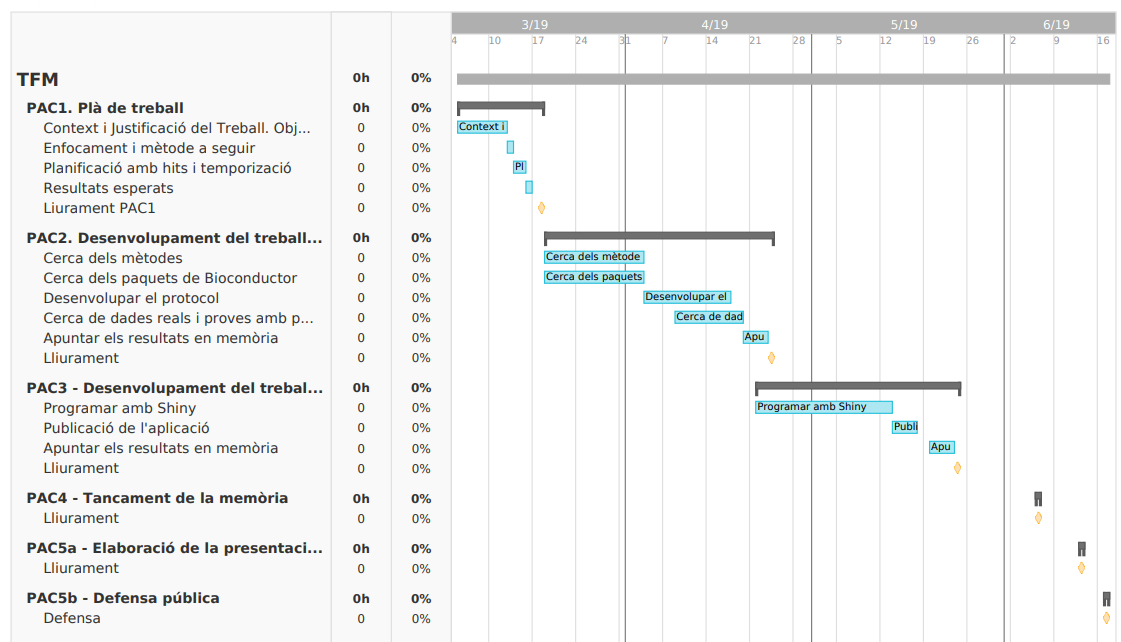
\includegraphics[width=0.9\textwidth]{GanttPlot}
\end{figure}

\begin{figure}[H]
\caption{Gantt List}
\centering
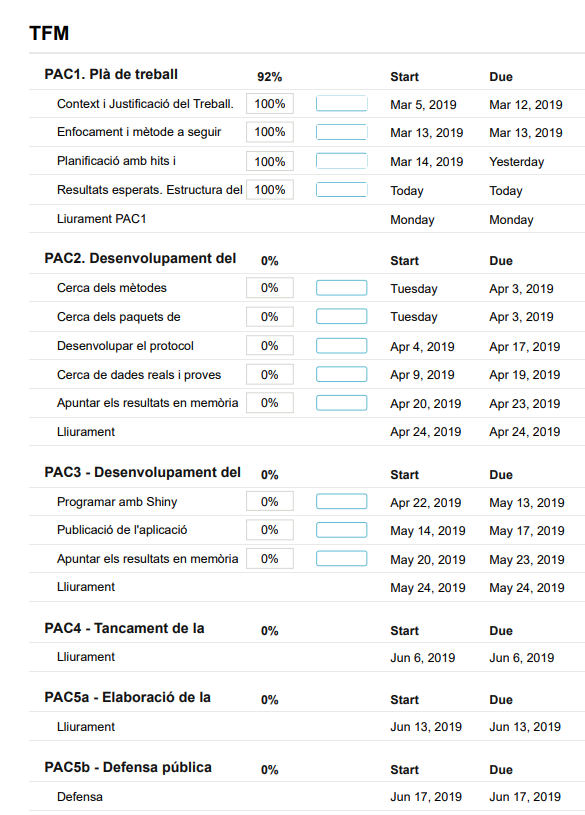
\includegraphics[width=0.9\textwidth]{GanttList}
\end{figure}


\begin{figure}[H]
\caption{Maig}
\centering
\includegraphics[width=0.9\textwidth]{Calender1_March}
\end{figure}


\begin{figure}[H]
\caption{Abril}
\centering
\includegraphics[width=0.9\textwidth]{Calender2_April}
\end{figure}

\begin{figure}[H]
\caption{Mai}
\centering
\includegraphics[width=0.9\textwidth]{Calender3_May}
\end{figure}

\subsection{Hits}
Els hits estan definits pel plà docent:

\begin{center}
 \begin{tabular}{||c | l | c | c||} 
 \hline
 Activitat & Nom d'activitat & Data d'inici & Data d'entrega  \\ [0.5ex] 
 \hline\hline
 PAC0 & Definició dels continguts del treball & 20/02/19 & \cellcolor[HTML]{AA0044} 04/03/2019 \\ 
 \hline
 PAC1 & Pla de treball & 05/03/19 & \cellcolor[HTML]{AA0044}18/03/19 \\
 \hline
 PAC2 & Desenvolupament del treball - Fase 1 & 19/03/19 &\cellcolor[HTML]{AA0044} 24/04/19 \\
 \hline
 PAC3 & Desenvolupament del treball - Fase 2 &  25/04/19 &\cellcolor[HTML]{AA0044} 20/05/19 \\
 \hline
 PAC4 & PAC4 - Tancament de la memòria & 21/05/19 &\cellcolor[HTML]{AA0044} 05/06/19 \\
 \hline
 PAC5a & PAC5a - Elaboració de la presentació & 06/06/19 &\cellcolor[HTML]{AA0044} 13/06/19 \\ 
  \hline
 PAC5b & PAC5b - Defensa pública & 17/06/19 &\cellcolor[HTML]{AA0044} 26/06/19 \\[1ex] 
 \hline
\end{tabular}
\end{center}

\subsection{Análisis de riscs}
He ellegit aquest tema perquè la creació  d'una applicació web amb shiny és un tema nou per a mi que m'agradaria aprendre. D'una banda és un desafiament personal per a mi però també representa un risc perquè alguns funcionament del Shiny no seràn obvis i necesitaràn una cerca intensiva de solucions.  L'altre factor del risc podria ser la gran quantitat d'informació sobre el tema de pathways tant en marc teòric com en marc pràctic dels paquets disponibles per fer l'anàlisi. Aquí estarà precís fer decisions aportunas i ràpides i no desviar l'atenció del objectiu principal. Podem resumir els factors del risc de forma següent:
\begin{enumerate}
\item No trobar els paquets adequats;
\item Trobar gran quantitat dels paquets que ofereixen estadístiques diferents. Cosa que dificultarà se sellecció de les estadístiques adequades;
\item Problemes amb creació de l'aplicació amb Shiny perquè serà el primer contacte amb Shiny. Aquí poden apareixer problemes inprevistes la solució dels quals implicarà una cerca intensiva de solucions en web i forums dedicats a Shiny;
\item Dificultats a l'hora de publicació de l'aplicació.  Hi ha diferents opcions de publicació d'aplicació: amb shinyapps.io i amb servidor Shiny. La primera opció és mes preferida perque no implica ni creació del servidor ni la seva configuració especial. La creació d'un servidor implicarà els costos economics que van a la direció contraria de l'objectiu de fer l'aplicació gratuita.  La opció de shinyapps.io però pot ser inviable perque es podran pruduir errors inesperats  que nececitaràn el control sobre el servidor cosa que shinyapps.io no ofereix (\href{https://groups.google.com/forum/#!msg/shinyapps-users/QRydNubnMQA/kJBxwUIJCgAJ)}{vegeuun exemple aquí}. 
\item Els imprevistos personals.
\end{enumerate}

\section{Resultats esperats}
\subsection{Plà de treball}
Amb aquest document es preten estructurar el projecte,  definir els objectius i assignar les tasques de tal manera que l'objectiu es pot aconseguir a temps d'entrega establert. Es tracta d'identicar els possibles problemes que poden influir en el cimplement temporal de les tasques definides. És la primera valoració del ptojecte desde perspectives diferents.

\subsection{Memòria}

Els mètodes i la seva implementació via programmari R han de ser documentats per fer el prcès de creació el més reproducible possible. Amb la memòria es preten documentar de manera estructurada els pasos fets per cumplir els objectius. També la memòria inluirà l'ús detallat del producte (Aplicació Shimy).

\subsection{Producte}
Amb aquest treball de màster es preten crear una aplicació Shiny que basarà en últims avenços teòrics en àmbit de l'anàlisi de les rutes. També haurà de proporcionar un interfície d'ús fàcil i a més a més ser gratuit. Els resultats obtinguts amb l'aplicació hauràn de tenir la qualitat suficiente per poder ser usats en una publicació scientífica.

Ja he començat ''jugar'' amb Shiny i he creat la primera visió de l'aplicació que servirà com a graella:

\begin{figure}[H]
\caption{Disseny de l'aplicació}
\centering
\includegraphics[width=0.9\textwidth]{App1}
\end{figure}

\begin{figure}[h!]
  \centering
  \begin{subfigure}[b]{0.4\linewidth}
    \includegraphics[width=\linewidth]{App2a}
    \caption{Go Analysis}
  \end{subfigure}
  \begin{subfigure}[b]{0.4\linewidth}
    \includegraphics[width=\linewidth]{App2b}
    \caption{KEGG Analysis}
  \end{subfigure}
    \begin{subfigure}[b]{0.4\linewidth}
    \includegraphics[width=\linewidth]{App2c}
    \caption{Reactome Analysis}
  \end{subfigure}
  \caption{Les anàlisis disponibles}
  \label{fig:coutput}
\end{figure}

 
\begin{figure}
\caption{Exemple del disseny}
\centering
\includegraphics[width=0.9\textwidth]{App3}
\end{figure}


\subsection{Presentació virtual}
El resultat de feina haurà de ser presentat davant un tribunall que valorarà l'esforç fet i a més la qualitat del producte conseguit.

\subsection{Autoevaluació del projecte}
En curt termini gairebe mai es pot conseguir que el resultat sigui perfecte. Aquí s'haurà d'indicar tan deficniencies com les vies de millora sobre el producte prsentat.

\section{Estructuració del projecte}

L'estructura del projecte està condicionada per el plà docent i inclou els components següents:

\begin{itemize}
\item Memòria del projecte
\item El producte conseguit
\item Presentacó dels mètodes utilitzats i del producte amb les seves characterístiques tècniques i pràctiques
\item Defensa del Treball davant el tribunal.
\end{itemize}

La memòria consistirà en descripció estructurada de les conceptes teòrics relacionats amb l'anàlisi de rutes. També incluira la descripció de l'aplicació i el protocol del seu ús. Aquí s'indicarà si tots els objectius eren aconseguits. També es farà autoevaluació per comentar els problemes no resolts (si n'hi ha) i possibilitats de millora. 

El producte obtingut es farà accesible on line en una de les vies idicades: o bé via shinyapps.io o bé via un servidor. Aquest producte ha de contenir eines per dur a terme l'anàlisi de les rutes i ha de ser capaç de crear un \textit{output} amb una qualitat apta per a una publicació scientífica. Què vol dir un rigor metodològic adequat i la qualitat de presentació/visualització dels resultats.

Finalment la memòria i el producte estaràn resumits en una presentació amb contingut per a  maximal 20 minunts d'intervenció oral. Aquí s'incluirà la descripció del \textit{pipeline} elaborat i  example pràctit d'anàlisi amb la aplicació. S'icluiran les captres de pantalla dels components principals de l'aplicació junts amb les tables i gràfics generats durant l'anàlisi de les dades de prova. 

Últimament es farà la defensa pública davant de tribunal.

Durant tot el procès s'haurà d'entregar informes de seguiment com a via per exposar el progrès de treball al professor responsable. Les sugerències del professor s'incorporaràn al  desenvolupament de l'aplicació.

\bibliography{references}
\bibliographystyle{apalike}
\end{document}





































